\documentclass[]{article}
\usepackage[utf8]{inputenc}
\usepackage[ngerman]{babel}
\usepackage[T1]{fontenc}
\usepackage{%
	ngerman,
	ae,
	times,  %% hier kann man die Schriftart einstellen
	graphicx,
	url,
	scrlayer-scrpage,
	lastpage,
	mathtools,
	geometry,
	multicol,
	cancel,
	xcolor,
	nicematrix,
	xfrac,
	tikz,
	pgfplots,
	amsmath,
	colortbl,
	centernot,
	dsfont,
	textgreek,
	icomma,
	pdfpages,
	kvmap}
\usepackage[thinlines]{easybmat}
\usetikzlibrary{datavisualization}
\usetikzlibrary{datavisualization.formats.functions}
\usetikzlibrary{intersections}
\pgfplotsset{compat=1.17}
\newcommand{\del}[1]{\cancel{~#1~}}
\NiceMatrixOptions{ last-col,code-for-last-col = \color{blue}\scriptstyle,light-syntax}
\newlength\dlf
\newcommand\alignedhighlight[3]{
  % #1 = color
  % #2 = before alignment
  % #3 = after alignment
  &
  \begingroup
  \settowidth\dlf{$\displaystyle #2$}
  \addtolength\dlf{\fboxsep+\fboxrule}
  \hspace{-\dlf}
  \fcolorbox{#1}{#1}{$\displaystyle #2 #3$}
  \endgroup
}
\newcommand{\reference}[1]{ \text{\small{\textcolor{blue}{(#1)}}} }

\newcommand{\topic}{Grundlagen Technische Informatik}
\newcommand{\subtopic}{Übung 1}
\newcommand{\authors}{Nils Helming}

%Head and Footnotes
\setlength{\headheight}{2.1\baselineskip} %baselineskip = minimum distance bbetween the bottom of one line to another.
\geometry{bottom = 3cm}
\setlength{\headsep}{\baselineskip}
\ihead[\topic\hrule]{\topic\hrule}
\chead[\subtopic\\~]{\subtopic\\~}
\ohead[\authors\\~]{\authors\\~}
\ifoot[~]{~}
\cfoot[~]{~}
\ofoot[Seite \thepage~von \pageref{LastPage}]{Seite \thepage~von \pageref{LastPage}}

%Paragraph spacings
\setlength{\parindent}{0em} %em = with of an 'M'
\setlength{\parskip}{1ex} %ex = height of an 'x'


\newcommand{\V}{\lor}
\newcommand{\A}{\land}
\newcommand{\T}[1]{\overline{#1}}
\newcommand{\eq}{\Leftrightarrow}
\newcommand{\rarr}{\Rightarrow}
\newcommand{\red}[1]{\textcolor{red}{#1}}

\newcommand{\unit}[1]{\text{#1}}
\newcommand{\fracunit}[2]{\frac{\unit{#1}}{\unit{#2}}}
\newcommand{\textsq}[1]{\ensuremath{\text{#1}^2}}
\newcommand{\textpow}[2]{\ensuremath{\text{#1}^{#2}}}
\newcommand{\tdot}{\ensuremath{\cdot}}


\begin{document}
\section*{Aufgabe 1:}
\subsection*{a)}
	\begin{center}
		\begin{kvmap}
			\begin{kvmatrix}{A,C,B}
				0 & 1 & \mathbf{1} & 0\\
				\mathbf{1} & 1 & 0 & 0\\
			\end{kvmatrix}
			\bundle[color=red]{1}{0}{2}{0}%{L}{T}{R}{B}
			\bundle[color=red]{0}{1}{1}{1}%{L}{T}{R}{B}
			\bundle[color=blue, reducespace=3pt]{1}{0}{1}{1}%{L}{T}{R}{B}
		\end{kvmap}
	\end{center}
	\begin{align*}
		Y = C\T{B} \V \T{A}B
	\end{align*}
\subsection*{b)}
	Der Aufwand ist hier $6$, da wir zwei UND-Verknüpfungen mit zwei Eingängen haben ($2\cdot 2$) und eine ODER-Verknüpfung mit zwei Eingängen haben ($1\cdot 2$). Also insgesamt $6$ Eingänge.
\subsection*{c)}
	Die DNF in diesem Fall würde aus insgesamt $4$ UND-Verknüpfungen mit jeweils $3$ Eingängen, wessen $4$ Ergebnisse dann in eine ODER-Verknüpfung eingegeben werden würde. Also haben wir einen Aufwand von $4\cdot 3 + 1\cdot 4 = 16$.

\section*{Aufgabe 2:}
\subsection*{a)}
	\begin{center}
		\begin{kvmap}
			\begin{kvmatrix}{D,A,C,B}
				\mathbf{1} & 0 & 0 & 0\\
				0 & 0 & \mathbf{1} & 0\\
				1 & \mathbf{1} & 0 & \mathbf{1}\\
				1 & 0 & 0 & 0\\
			\end{kvmatrix}
			\bundle[color=red]{2}{1}{2}{1}%{L}{T}{R}{B}
			\bundle[color=green, reducespace=4pt]{0}{2}{1}{2}%{L}{T}{R}{B}
			\bundle[color=blue, reducespace=2pt]{0}{2}{0}{3}%{L}{T}{R}{B}

			\draw[kvbundle,red] (00.north west) |- (00.south);
			\draw[kvbundle,red] (00.north east) |- (00.south);
			\draw[kvbundle,red] (03.south west) |- (03.north);
			\draw[kvbundle,red] (03.south east) |- (03.north);

			\draw[kvbundle,red] (02.north west) -| (02.east);
			\draw[kvbundle,red] (02.south west) -| (02.east);
			\draw[kvbundle,red] (32.north east) -| (32.west);
			\draw[kvbundle,red] (32.south east) -| (32.west);
		\end{kvmap}
	\end{center}
	\begin{align*}
		Y = \T{A}\T{B}\T{D} \V AB\T{C}D \V BC\T{D} \V \T{A}BC
	\end{align*}
\subsection*{b)}
	\begin{center}
		\begin{kvmap}
			\begin{kvmatrix}{D,A,C,B}
				1 & 0 & 0 & 0\\
				0 & 0 & 1 & 0\\
				1 & 1 & \mathbf{0} & 1\\
				1 & \mathbf{0} & 0 & \mathbf{0}\\
			\end{kvmatrix}
			\bundle[color=green, reducespace=2pt]{2}{2}{2}{3}%{L}{T}{R}{B}
			\bundle[color=red, reducespace=2pt]{3}{0}{3}{1}%{L}{T}{R}{B}
			\bundle[color=red, reducespace=2pt]{0}{1}{1}{1}%{L}{T}{R}{B}
			\bundle[color=blue, reducespace=4pt]{1}{0}{1}{1}%{L}{T}{R}{B}

			\draw[kvbundle,blue] (31.north east) -| (31.west);
			\draw[kvbundle,blue] (31.south east) -| (31.west);
			\draw[kvbundle,blue] (01.north west) -| (01.east);
			\draw[kvbundle,blue] (01.south west) -| (01.east);

			\draw[kvbundle,red] (10.north west) |- (20.south west);
			\draw[kvbundle,red] (20.south west) -| (20.north east);
			\draw[kvbundle,red] (13.south west) |- (23.north west);
			\draw[kvbundle,red] (23.north west) -| (23.south east);

			\draw[kvbundle,blue] (20.north west) |- (30.south west);
			\draw[kvbundle,blue] (30.south west) -| (30.north east);
			\draw[kvbundle,blue] (23.south west) |- (33.north west);
			\draw[kvbundle,blue] (33.north west) -| (33.south east);
		\end{kvmap}
	\end{center}
	\begin{align*}
		\T{Y}&= D \T{B} \V A\T{B} \V ACD \V A\T{C}\T{D} \V \T{A}B\T{C}\\
		Y &= (\T{D} \V B) \A (\T{A}\V B) \A (\T{A} \V \T{C} \V \T{D}) \A (\T{A} \V C \V D) \A (A \V \T{B} \V C)
	\end{align*}

\section*{Aufgabe 3:}
\subsection*{a) (DMF)}
	\begin{center}
		\begin{kvmap}
			\begin{kvmatrix}{B,D,A,C}
				0 & \mathbf{1} & 0 & 0\\
				0 & 1 & * & 0\\
				* & 1 & 0 & \mathbf{1}\\
				0 & * & \mathbf{1} & 0\\
			\end{kvmatrix}
			\bundle[color=red]{1}{0}{1}{3}%{L}{T}{R}{B}
			\bundle[color=blue, reducespace=2pt]{1}{1}{2}{1}%{L}{T}{R}{B}
			\bundle[color=blue, reducespace=2pt]{0}{2}{1}{2}%{L}{T}{R}{B}
			\bundle[color=blue, reducespace=2pt]{1}{3}{2}{3}%{L}{T}{R}{B}

			\draw[kvbundle,red] (02.north west) -| (02.east);
			\draw[kvbundle,red] (02.south west) -| (02.east);
			\draw[kvbundle,red] (32.south east) -| (32.west);
			\draw[kvbundle,red] (32.north east) -| (32.west);
		\end{kvmap}
	\end{center}
	\begin{align*}
		Y = \T{B}D \V AC\T{D} \V A\T{C}D
	\end{align*}

\subsection*{a) (KMF)}
	\begin{center}
		\begin{kvmap}
			\begin{kvmatrix}{B,D,A,C}
				0 & 1 & \mathbf{0} & 0\\
				0 & 1 & * & 0\\
				* & 1 & \mathbf{0} & 1\\
				0 & * & 1 & \mathbf{0}\\
			\end{kvmatrix}
			\bundle[color=blue, reducespace=2pt]{0}{0}{0}{3}%{L}{T}{R}{B}
			\bundle[color=blue, reducespace=2pt]{2}{0}{3}{1}%{L}{T}{R}{B}
			\bundle[color=red, reducespace=0pt]{2}{1}{2}{2}%{L}{T}{R}{B}

			% 00,01> ... <30,31
			\draw[kvbundle,red] (00.north west) -| (01.east);
			\draw[kvbundle,red] (01.south west) -| (01.east);
			\draw[kvbundle,red] (30.north east) -| (31.west);
			\draw[kvbundle,red] (31.south east) -| (31.west);

			% 03> ... <33
			\draw[kvbundle,red] (03.north west) -| (03.east);
			\draw[kvbundle,red] (03.south west) -| (03.east);
			\draw[kvbundle,red] (33.north east) -| (33.west);
			\draw[kvbundle,red] (33.south east) -| (33.west);
		\end{kvmap}
	\end{center}
	\begin{align*}
		\T{Y} &= \T{A}B \V BCD \V \T{C}\T{D} \V \T{B}\T{D}\\
		Y &= (A\V\T{B}) \A (\T{B}\V \T{C}\V \T{D}) \A (C\V D) \A (B\V D)\\
	\end{align*}
\subsection*{b)}
	Der Aufwand der Disjunktiven Minimalform ist $2+3+3+3 = 11$.\\
	Der Aufwand der Konjunktiven Minimalform ist $2+3+2+2+4 = 13$.\\

\subsection*{c)}
	Zusätzlich der Ursprünglichen form, muss der Disjunktiven Minimalform noch ein Term hinzugefügt werden, um Hazard-frei zu werden:
	$A \T{B} C$
	\begin{align*}
		Y = \T{B}D \V AC\T{D} \V A\T{C}D \V A \T{B} C
	\end{align*}

	Zusätzlich der Ursprünglichen Form, muss der Konjunktiven Minimalform  noch ein Term hinzugefügt werden, um Hazard-frei zu werden:
	$A \V D$
	\begin{align*}
		Y &= (A\V\T{B}) \A (\T{B}\V \T{C}\V \T{D}) \A (C\V D) \A (B\V D) \A (A \V D)\\
	\end{align*}
	Alternativ hätte auch schon zu beginn eine Hazard-Freie Minimalform gewählt werden können.
	\begin{align*}
		Y &= (A\V\T{B}) \A (\T{B}\V \T{C}\V \T{D}) \A (C\V D) \A (A \V D)\\
	\end{align*}

\subsection*{d)}
	DMF + Hazard-frei: $2+3+3+3+4 = 15$\\
	KMF + Hazard-frei: $3+3+2+2+2+5 = 16$\\
	KMF + Hazard-frei (version 2): $3+3+2+2+2+5 = 13$\\

\section*{Zusatzaufgabe (Zu Aufgabe 3)}
mit Logikbausteinen Realisieren: (DMF aus Aufgabe 3a) Vorhanden sind Inverter und NAND-Bausteine.
\begin{align*}
	Y &= \T{B}D \V AC\T{D} \V A\T{C}D \V A \T{B} C \\
	 &= \T{\T{   \T{B}D \V AC\T{D} \V A\T{C}D \V A \T{B} C }} \\
	\text{DeMorgan:} &= \T{\T{   \T{B}D} \A  \T{AC\T{D}} \A \T{A\T{C}D} \A \T{A \T{B} C }} \\
\end{align*}
Chip 7404 ist enthält 6 Inverter - Drei davon benötigen wir. Also einmal 7404.\\
Chip 7410 ist enthält 3 NAND mit drei Eingängen - Vier davon benötigen wir. Also zwei 7410.\\
\begin{center}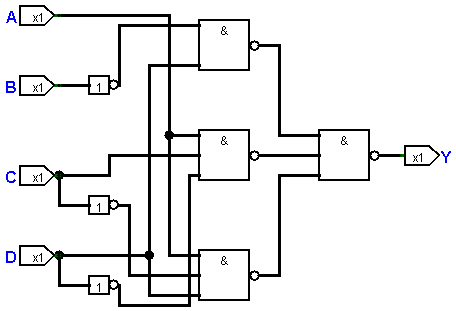
\includegraphics[scale=0.5]{Bilder/Zusatz.png}\end{center}
\begin{center}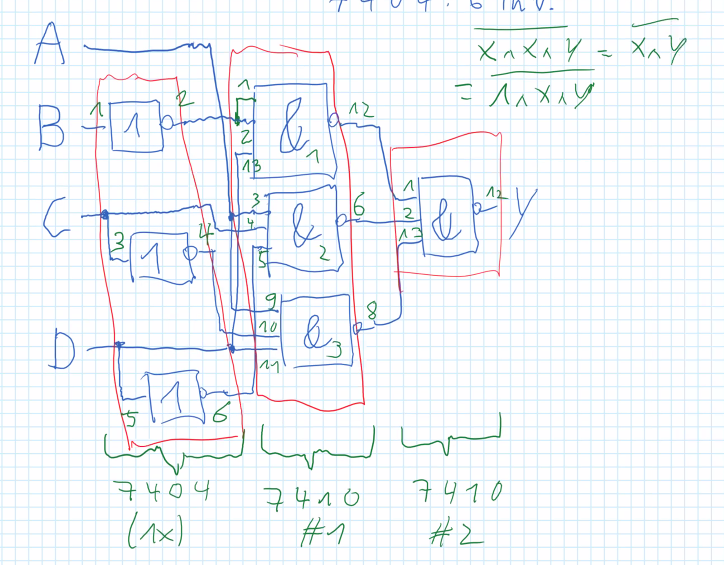
\includegraphics[scale=0.5]{Bilder/Skizze_Zusatz.png}\end{center}
\begin{center}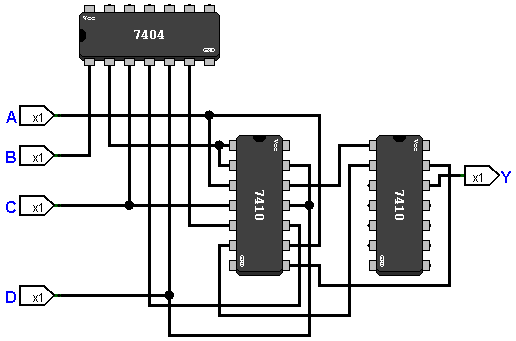
\includegraphics[scale=0.5]{Bilder/Bausteine.png}\end{center}
\end{document}